\section{Co-design of estimation and control}
\label{sec:codesign}
In a traditional control system, %such as the one shown in Fig.~\ref{fig:traditionalCE}, 
the controller is unaware of the implementation details of the estimation module and the estimation module is unaware of the requirements of the controller.
For example, the design of a feedback controller might not take into account the fact that obtaining a state estimate from a video feed will take a non-negligible amount of time, which we refer to as the estimation delay.
Conversely, the design of the perception and estimation might not in general take into account the varying real-time constraints that the controlled system must satisfy. %, and instead always run-to-completion compute its estimates.
In order to improve performance of real-time closed loop systems using computationally and power limited platforms, we propose the \emph{co-design} of estimation and control.
The co-design involves using a \emph{contract-based framework} for both estimator and controller.
Namely, the controller requests the estimator to provide a state estimate within a certain deadline $\delta$ seconds and with a certain error bound $\epsilon$.
We refer to the tuple $(\delta,\epsilon)$ as the \emph{contract} between controller and estimator. 
The estimator then provides an estimate that respects the contract.
By requesting estimates with varying contracts during system operation, the controller is able to adapt the closed-loop system performance in real-time according to the current condition of the physical system.
For example, it can decide when an estimate is needed fast (but usually with higher error), and when a more accurate estimate is needed (but with greater delay). Note, the $(\delta,\epsilon)$ contract can also be thought of as setting an operating mode for the perception-and-estimation algorithm. A high-level view of this setup is shown in Fig.~\ref{fig:codesignedCE}.

To ensure that the estimator can respect the contract (alternatively, that the controller is only requesting contracts that can be fulfilled by the estimator), the estimator is profiled off-line.
Namely, the estimator's parameters are varied and for each setting of the parameters, it is run on a \emph{profiling data set}. 
This yields a finite set of $(\delta,\epsilon)$ values, each one corresponding to a setting of the parameters.
These values can be plotted on a curve, which we call the \emph{error-delay curve} made up of discrete points, $\de$, represented by the set $\Delta$. Examples of such a curve are shown in Figs. \ref{fig:eps_delta_toy} and \ref{fig:svo_error_delay}.
The detailed procedure for obtaining such a curve for a perception based algorithms is given in Section \ref{delayErrorCurve}.
%Section \ref{discussion} discusses the applicability of this contract-based approach to state estimation and further extensions.

At run-time, when the estimator receives a $\de$ contract request from the controller, it can adapt its execution paths to respect the contract, namely, to provide a state estimate in real-time within the requested error bound $\epsilon$, and within the requested deadline $\delta$.

In addition, the controller is designed with the knowledge of the error-delay curve of the estimation algorithm, and requests contracts from that curve.
Thus, the error-delay curve constitutes the \textit{interface} between controller and estimator.
This gives the controller the ability to leverage the flexible nature of the estimation algorithm to maximize some performance measure of control performance. %\todo[inline]{Might want to avoid mentioning \emph{separability principle}}

Fig.~\ref{fig:fullcodesignedCE} shows the closed loop architecture in a system with co-design of the estimator and controller.
In the co-designed system as presented in this paper, the controller can make the estimation algorithm switch to lower or higher time (and/or energy) consuming modes based on the control objective at the current time step.
The main components of the co-design architecture are a contract based perception-and-estimation algorithm, a robust control algorithm that computes an input to be sent to the physical system being controller as well as the operating mode for the contract time estimator, and the interface between them. More details on these components are in the following sections.

%\begin{figure*}[t]
%	\centering
%	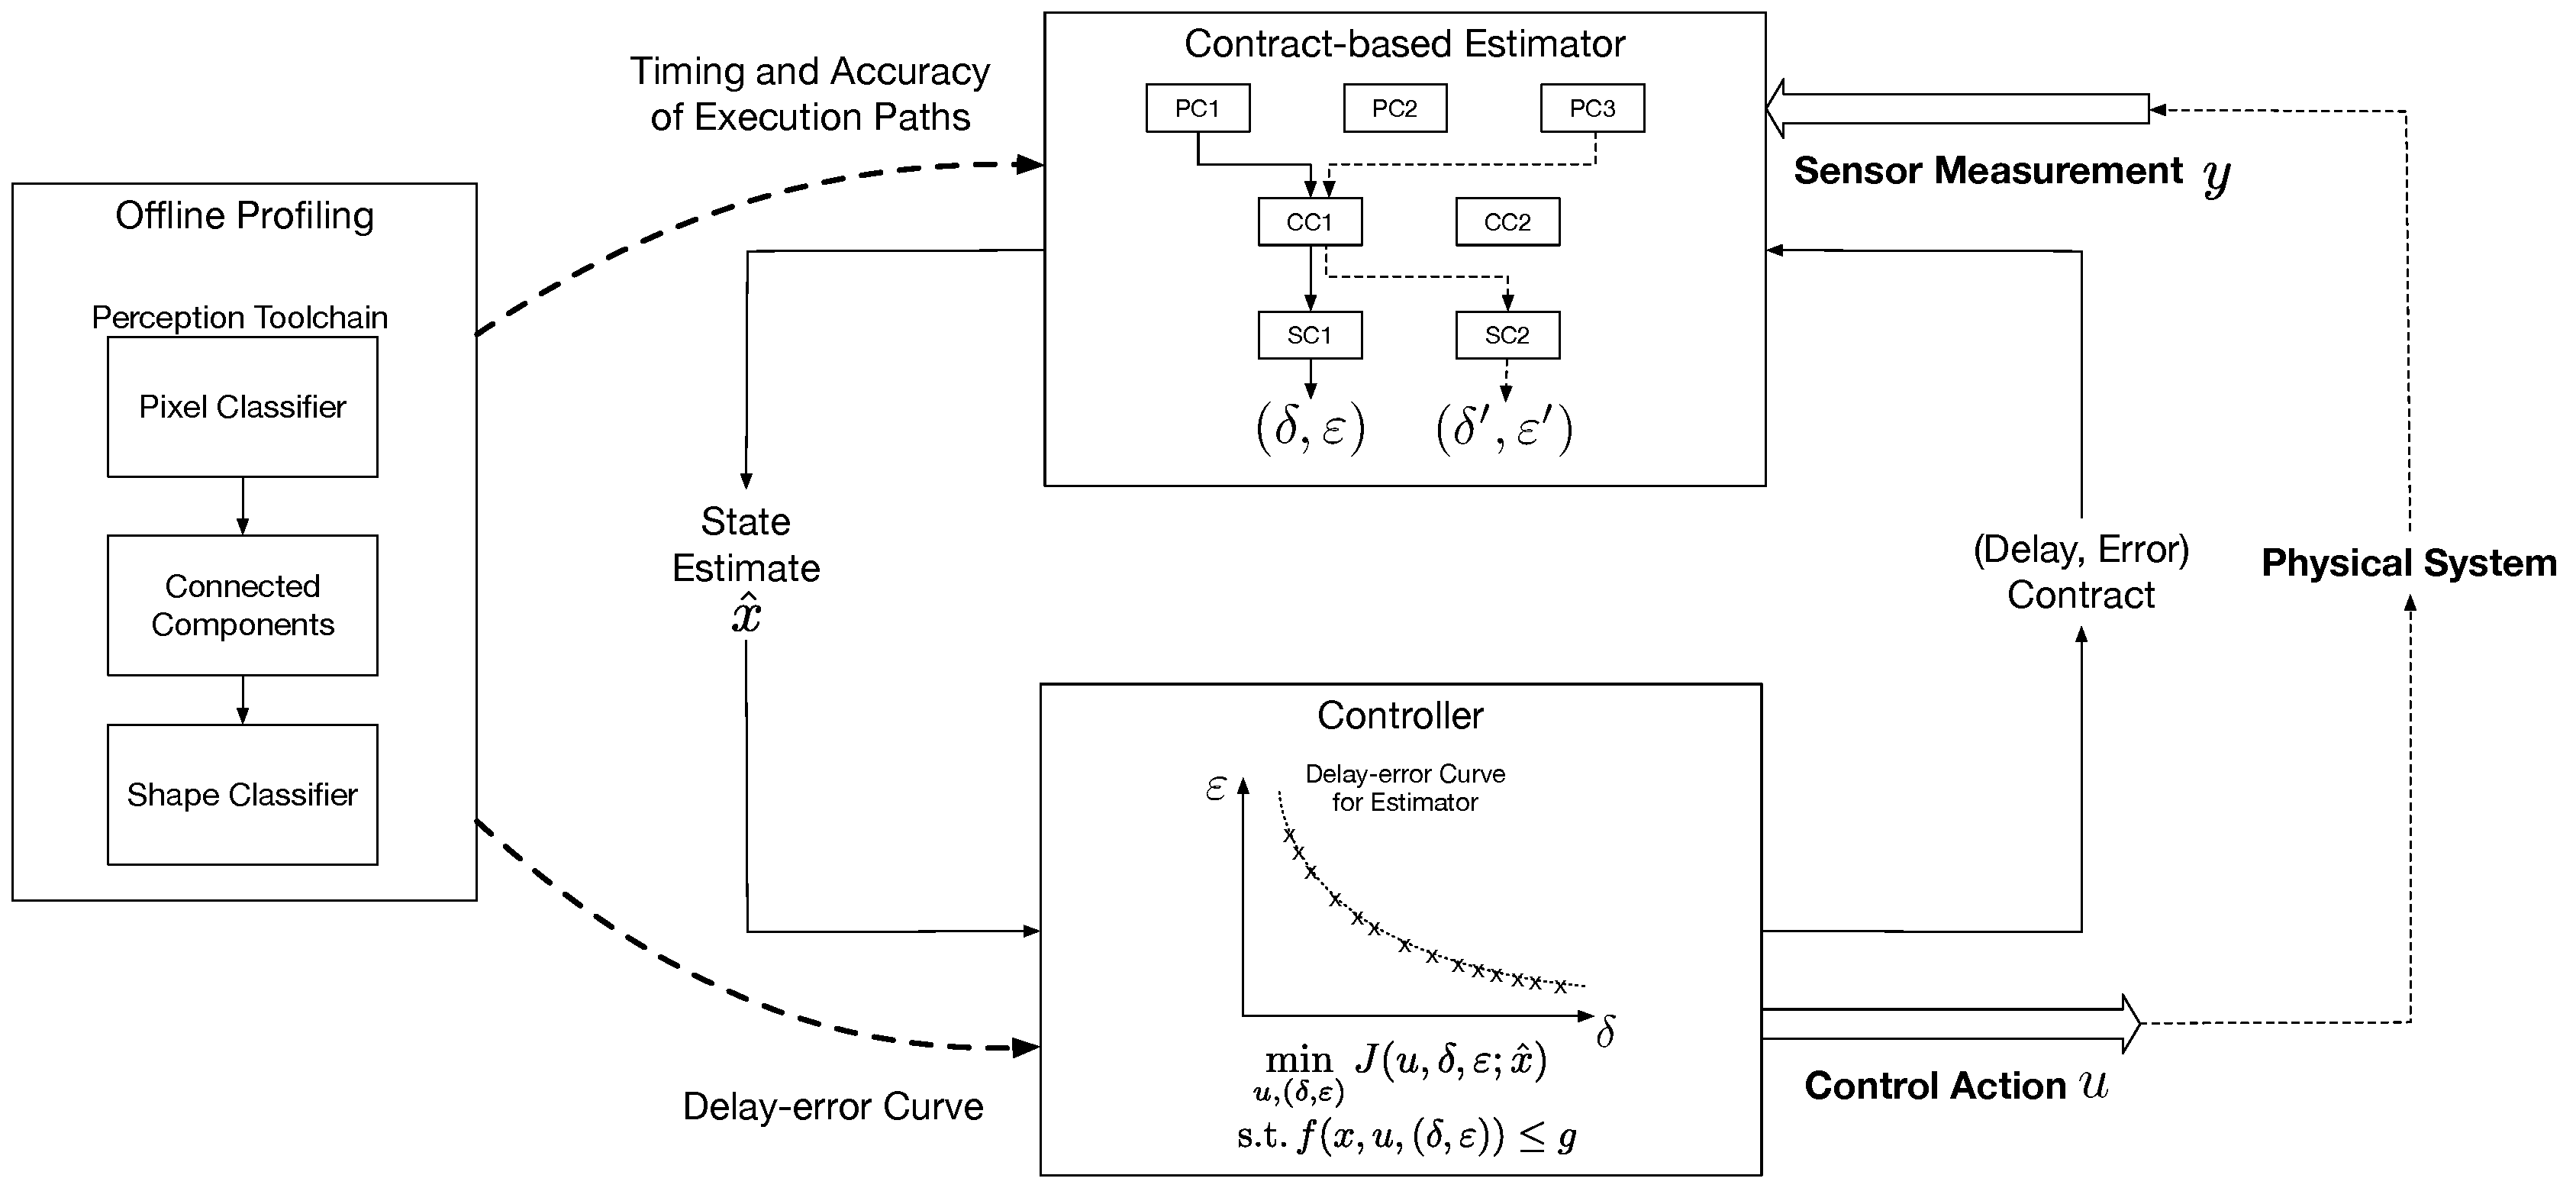
\includegraphics[width=0.9\textwidth]{figures/omnigraffle_figures/process_figure2}
%	\caption{Contract-based estimator and controller}
%	\label{fig:fullcodesignedCE}
%\end{figure*}
\subsection{Contract based perception algorithms}

%In order to maximize the efficiency of the computation and control system,
A contract based perception-and-estimation algorithm can operate at different deadlines and provide a usable solution for the control algorithm to operate on. This flexible operation is achieved by composing the algorithm of functional blocks that have different execution times and result in different qualities of outputs. 

% MOVE TO RELATED
%Note that this problem is different from that of composing multiple anytime algorithms together \cite{zilbersteinAImag}. Anytime algorithms \cite{boddy} have a well defined computation time versus quality tradeoff, but in our case we are composing together blocks that are individually run-to-completion and in most cases do not have a well defined intermediate measurable quality.

%Figure \ref{fig:RT_bs} shows 
An example is a Computer Vision (CV) based Object recognition algorithm which is composed of different functional blocks of varying execution time which result in a different accuracy when linked together to provide the functionality of an object recognition algorithm. E.g. the pixel classifier in the first stage of such a CV algorithm could be a Gaussian Mixture Model with 2, 4, or 6 components, with more components providing better classification performance (over-fitting is ruled out by cross-validation) at the cost of more computation time. Functions with similar characteristics like example above, when profiled extensively offline and composed in the right order at run-time can be used to compose a contract time anytime perception and estimation algorithm. More details follow in section \ref{delayErrorCurve}.

%The output of the pixel classifier, which is a binary image, can then be filtered and connected into objects using a variety of filters and connected component methods. Finally the connected objects have to pass through a shape classifier to ensure that we detect only the object of interest.

%.... \textbf{<more details here>}.

%This composition of individual components can be represented as a decision tree where edges are blocks of code and nodes are their intermediate outputs/input to the next stage. An extensive profiling stage at design time helps assign distributions for execution times to the edges and distributions for output quality to paths along the tree. At run-time, this knowledge of execution times and output quality distributions can be used to generate a composition to realize a given criteria. An example of a criteria is to maximise the expected quality while meeting the given deadline with a high probability $\eta$.



%Given a decision tree with pre-profiled information about execution time distributions for edges and quality for paths, this optimization can be mapped to an integer programming problem for edge selection in the tree. This problem can be solved in a

%\textbf{<more details on the optimization here>}

\subsection{Interface between contract based perception and robust control}

For the control algorithm to be able to leverage the flexible nature of the contract based perception algorithm, it must have information about the computation time versus output quality trade-off that the contract based perception algorithm offers. An interface that achieves this is obtained by representing the profiled behaviour of the contract based algorithm to varying deadlines, as points on a perception quality versus deadline ($\delta, \epsilon$) curve, e.g. in Fig. \ref{fig:eps_delta_toy}.
With this profiled curve available to the controller at runtime, the exchange of information between the contract based perception-and-estimation algorithm and the control algorithm consists of the controller assigning a deadline ($\delta$), or a contract to the perception algorithm while expecting a bound on the error ($\epsilon$) of its output. The perception algorithm then returns an output after internally deciding the composition to best meet the deadline and the expected quality requirement. 
%While in many systems, assigning a contract for time and simultaneously expecting a minimum quality output may be an infeasible proposition, in this paper we only consider settings where neither the $\delta$ contract nor the $\epsilon$ bound are violated.
Through extensive offline profiling, we guarantee with a high degree of confidence that the contract based estimator does not violate the contract. This helps in formulating a control algorithm that provides mathematical guarantees on the feasibility of constraints for the safe operation and stability of the closed loop dynamic system as covered in section \ref{robustMPC}.

\subsection{Robust Control with contract based perception algorithm}

The control algorithm is designed to pick the best operating point for the estimator, or the right $\de$ contract to request from the perception and estimation algorithm. This is done based on the current state of the physical system to maximize a performance measure while being robust to the varying computation time and the varying estimation errors of the estimator with different contracts as is provides estimates to the controller. In section \ref{robustMPC} we present a control algorithm that achieves this while also guaranteeing feasibility of system constraints the stability of the closed loop system.






